\chapter{PRACTICAL CONSIDERATIONS}
\label{chap:application}

\section{Parameter Values}
\label{sec:parameters}
In this chapter, model parameters are discussed.
In the case that this model is run in conjunction with a kelp growth model and ocean model,
they will provide some of the necessary parameters.
Other parameters not coming from the kelp or ocean model can be found in the literature,
summarized in Table \ref{tab:params} and Table \ref{tab:petzold}.
Still, some parameters remain which are not well described in the literature.

\subsection{Simulation Parameters}
It is assumed that this model is run together with a kelp growth model such as described in \citep{broch_modelling_2012}, and an ocean model, as in \citep{wassmann_modelling_2006}.
Both models are assumed to use the same spatial grid, with $n_z$ discrete depth layers of thickness $dz_k$ for $k=1,\ldots,n_z$.
It is assumed that the horizontal spacing for both models is quite large, and the light model therefore uses a much finer horizontal resolution,
but retains the same vertical resolution as the encompassing calculations.
The ocean model provides current speed and direction over depth, which is used in calculating the kelp distribution.
The position of the sun and irradiance just below the surface of the water is also provided by the ocean model, which is used to generate the surface radiance boundary condition.
The ocean model should also provide an absorption coefficient for each depth layer, which may vary due to nutrient concentrations and biological specimens such as phytoplankton.
The kelp model is expected to provide super-individual data describing the population in each depth layer.
Then, \eqref{eqn:si_mean} and \eqref{eqn:si_std} are used to calculate length and orientation distributions, as described in Section \ref{sec:si}.

% TODO: Add data from Ole Jacob's student's thesis
\subsection{Parameters from Literature}
Given here is a table of parameter values found in the literature which are used in Chapter \Rom{\ref{chap:model_analysis}} to test this light model.
A few comments are in order.
No values were available for the absorptance of \textit{Saccharina latissima}, but a value for \textit{Macrocystis pyrifera} was found.
The surface irradiance from \cite{broch_modelling_2012} was given in terms of photons per second,
and was converted to \SI{}{\W\per\m\squared} according to \eqref{eqn:watts_photons}.
No data in the literature exist for the frond thickness, so a best estimate is provided.

\begin{table}
  \centering
  \caption{Parameter values.}
  %\begin{tabular}{p{2\textwidth/7} p{\textwidth/7} p{\textwidth/6} p{\textwidth/6} p{2\textwidth/7}}
  \begin{tabular}{lrrr}
    \toprule
    Parameter Name & Symbol & Value(s) & Citation \\ %& Notes \\
    \midrule
    Kelp absorptance & $A_k$ & 0.8 & \cite{colombo-pallotta_photosynthetic_2006} \\% & Actually for \textit{Macrocystis Pyrifera}\\
    Water absorption coefficient & $a_w$ & See Table \ref{tab:petzold} & \cite{petzold_volume_1972} \\%  & ? \\
    Scattering coefficient & $b$  & See Table \ref{tab:petzold} & \cite{petzold_volume_1972} \\%  & ? \\
    Volume scattering function & $\beta$ & tabulated & \cite{petzold_volume_1972,sokolov_parameterization_2010}, \\% & Currently using Petzold \\ 
    Frond thickness & $t$ & \SI{0.4}{\mm} & estimated \\
    Surface solar irradiance & $I_0$ & \SI{50}{\W\per\m\squared} & \cite{broch_modelling_2012}  \\% & Irradiance for maximal photosynthesis, converted from photons \\
    \bottomrule
  \end{tabular}
  \label{tab:params}
\end{table}

In \citep{petzold_volume_1972}, very detailed measurements of optical properties in various ocean waters are presented.
A few of those measurements are reproduced here, using the same site names as in the original report.
There are three categories of water provided: AUTEC is from Tongue of the Ocean, Bahama Islands,
and represents very clear, pure water; HAOCE is from offshore southern California, and represents a more average coastal region,
likely the most similar to water where kelp cultivation would occur; NUC data is from the San Diego Harbor, and represents very turbid water,
likely more so than one would expect to find in a seaweed farm.

\begin{table}
  \centering
  \caption{Field measurement data of optical properties in the ocean \cite{petzold_volume_1972}.
    The site names used in the original paper are used: AUTEC -- Bahamas, HAOCE -- Coastal southern California, NUC -- San Diego Harbor.
    Absorption, scattering, and attenuation coefficients ($a,b,c$) are given, and their ratios.
  }
  \begin{tabular}{lrrrrr}
    \toprule
    Site & $a (\mbox{m}^{-1})$ & $b (\mbox{m}^{-1})$ & $c(\mbox{m}^{-1} )$ & $a/c$ & $b/c$ \\
    \midrule
    % AUTEC 7 & $0.082$ & $0.117$ & $0.199$ & $0.412$ & $0.588$ \\
    AUTEC 8 & $0.114$ & $0.037$ & $0.151$ & $0.753$ & $0.247$ \\
    % AUTEC 9 & $0.122$ & $0.043$ & $0.165$ & $0.742$ & $0.258$ \\
    % HAOCE 5 & $0.195$ & $0.275$ & $0.47$ & $0.415$ & $0.585$ \\
    HAOCE 11 & $0.179$ & $0.219$ & $0.398$ & $0.449$ & $0.551$ \\
    NUC 2200 & $0.337$ & $1.583$ & $1.92$ & $0.176$ & $0.824$ \\
    % NUC 2040 & $0.366$ & $1.824$ & $2.19$ & $0.167$ & $0.833$ \\
    NUC 2240 & $0.125$ & $1.205$ & $1.33$ & $0.094$ & $0.906$ \\
    % Filtered Fresh & $0.093$ & $0.009$ & $0.102$ & $0.907$ & $0.093$ \\
    % Filtered Fresh + Scat.  & $0.138$ & $0.547$ & $0.685$ & $0.202$ & $0.798$ \\
    % Fresh + Scat. + Abs.& $0.764$ & $0.576$ & $1.34$ & $0.57$ & $0.43$ \\
    % As Delivered & $0.196$ & $1.284$ & $1.48$ & $0.133$ & $0.867$ \\
    % Filtered 40 min & $0.188$ & $0.407$ & $0.595$ & $0.315$ & $0.685$ \\
    % Filtered 1hr 40 min & $0.093$ & $0.081$ & $0.174$ & $0.537$ & $0.463$ \\
    % Filtered 18hr & $0.085$ & $0.008$ & $0.093$ & $0.909$ & $0.091$ \\
    \bottomrule
  \end{tabular}
  \label{tab:petzold}
\end{table}

\subsection{Frond Alignment Coefficient}
The \textit{frond alignment coefficient}, $\eta$, describes the dependence of frond alignment on current speed.
To the author's knowledge, no such parameter is available in the literature.
However, similar measurements have been made in the MACROSEA project by Norvik \cite{norvik_design_2017} to describe
the dependence of the elevation angle of the frond as a function of current speed.
In that study, artificial seaweed was designed, suitable for use in fresh water laboratory flumes without fear of degradation.
Using those synthetic kelp fronds, one could perform a simple experiment to determine the frond alignment coefficient, sketched here.

Fix a taught vertical rope or rod in the center of a flume, and attach the fronds to it with a short string which acts as the stipe.
To emulate the holdfast, the string should be tied tightly around the vertical rope or rod so as to prevent it from rotating at its attachment point,
giving the frond a preferred orientation from which it has to bend.
The preferred directions should be more or less evenly distributed.
A camera should be mounted directly over the vertical rope, pointed straight down.
If possible, a flourescent dye could be applied to the tip of the each frond to make their orientation more easily discernable in the recording.
Turn on the flume to several current speeds, recording a video or many snapshots for each.
If the fluorescent dye is applied, then a simple peak-finding image processing algorithm can be applied to locate the frond tips.
By preprocessing the image to a gray scale such that the color of the dye has the highest intensity,
the tip locations are located at local maxima.

Once the tip locations are determined, the azimuthal orientations can be calculated relative to the vertical line.
Data from all snapshots for the same current speed can be combined, and a von Mises distribution can be fitted to the combined data,
noting the best fit values of $\mu$ and $\kappa$.
Presumably, the best fit $\mu$ will be in the direction of current flow.
After repeating the procedure for several current speeds, $\kappa$ can be plotted as a function of current speed.
Then, an optimal value for the frond alignment coefficient $\eta$ can be found by fitting $\kappa = \eta\mu$ to the data.
It may, of course, turn out that this simple linear relationship does not hold, in which case a more appropriate description can be determined.

\section{Algorithm Parameters}
% TODO

\section{Computational Resources}
\subsection{CPU Time}
32 cores

\begin{figure}[H]
  \centering
  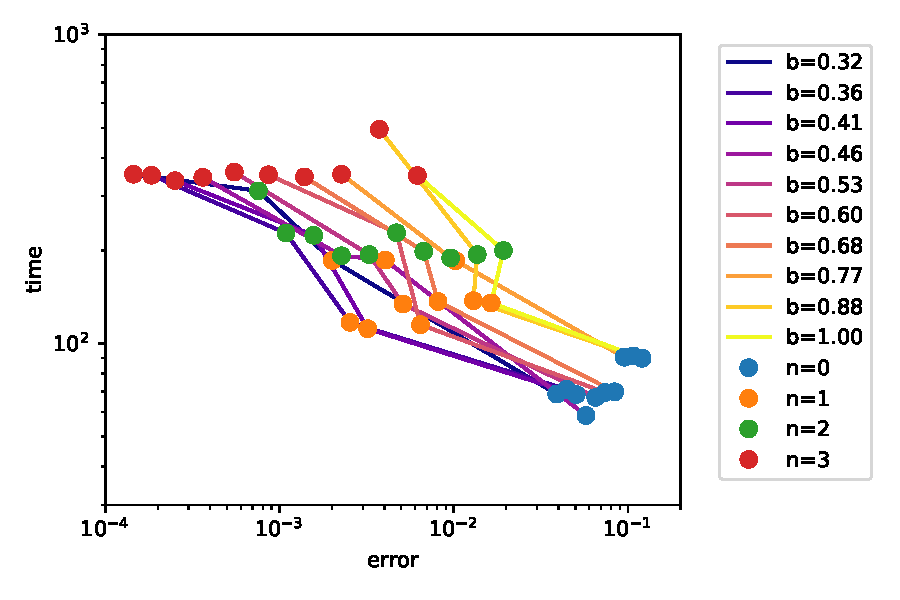
\includegraphics[width=5in]{mms_asym_err_time}
  \caption{mms asym err time, $n_s=64$, $n_a=8$}
  \label{fig:mms_asym_err_time}
\end{figure}

\begin{figure}[H]
  \centering
  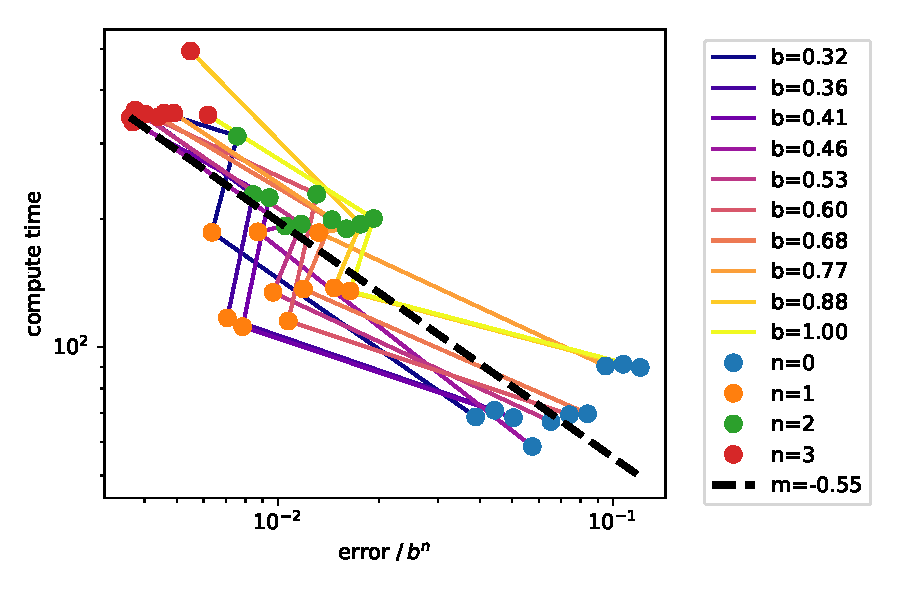
\includegraphics[width=5in]{mms_asym_err_time_collapsed}
  \caption{err time collapsed, $n_s=64$, $n_a=8$. $\varepsilon t^2 \propto b^n$}
  \label{fig:mms_asym_err_time_collapsed}
\end{figure}

\begin{figure}[H]
  \centering
  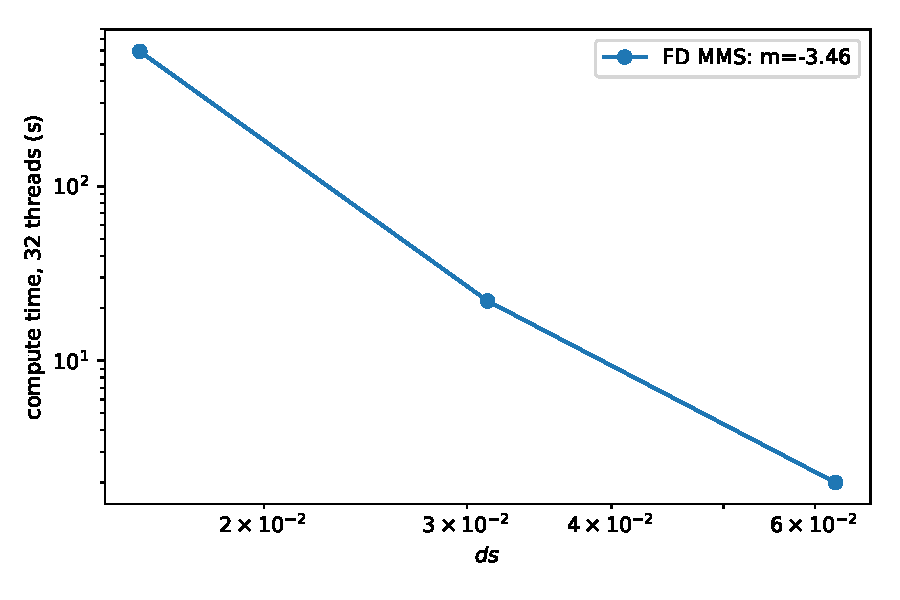
\includegraphics[width=5in]{fd_mms_time}
  \caption{mms asym err time, $n_s=64$, $n_a=8$}
  \label{fig:fd_mms_time}
\end{figure}

\begin{figure}[H]
  \centering
  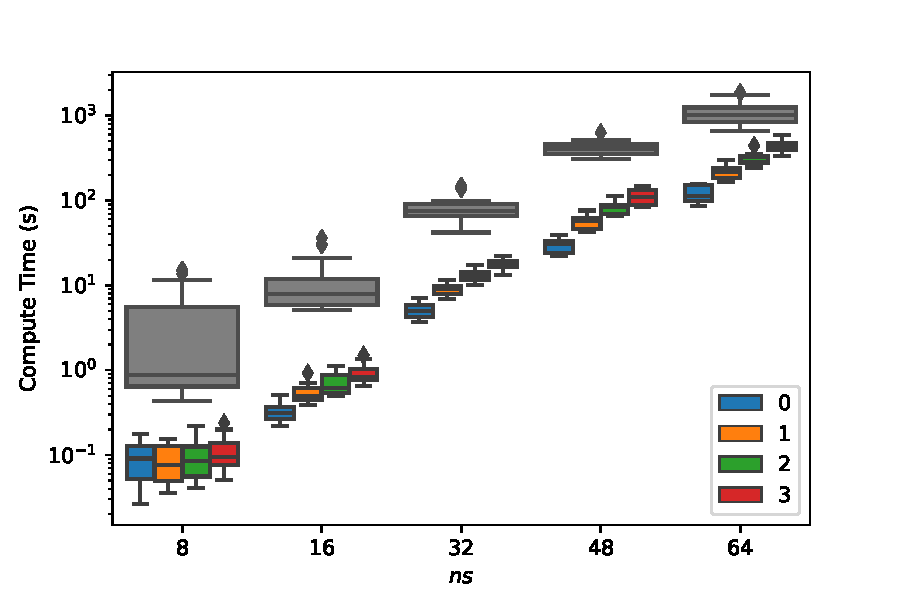
\includegraphics[width=5in]{compute_time_violin}
  \caption{mms asym err time}
  \label{fig:compute_time_violin}
\end{figure}

\subsection{Memory Usage}
\subsubsection{Single Matrix}
\begin{figure}[H]
  \centering
  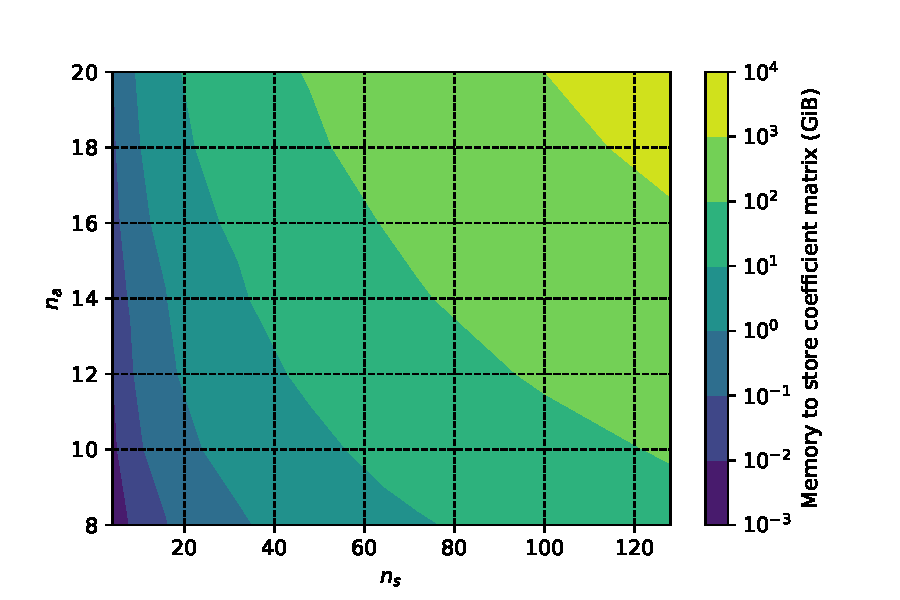
\includegraphics[width=5in]{memory_store}
  \caption{Memory to store one copy of the finite difference coefficient matrix}
  \label{fig:memory_store}
\end{figure}

\subsubsection{LIS Solution Memory Estimate}
\begin{figure}[H]
  \centering
  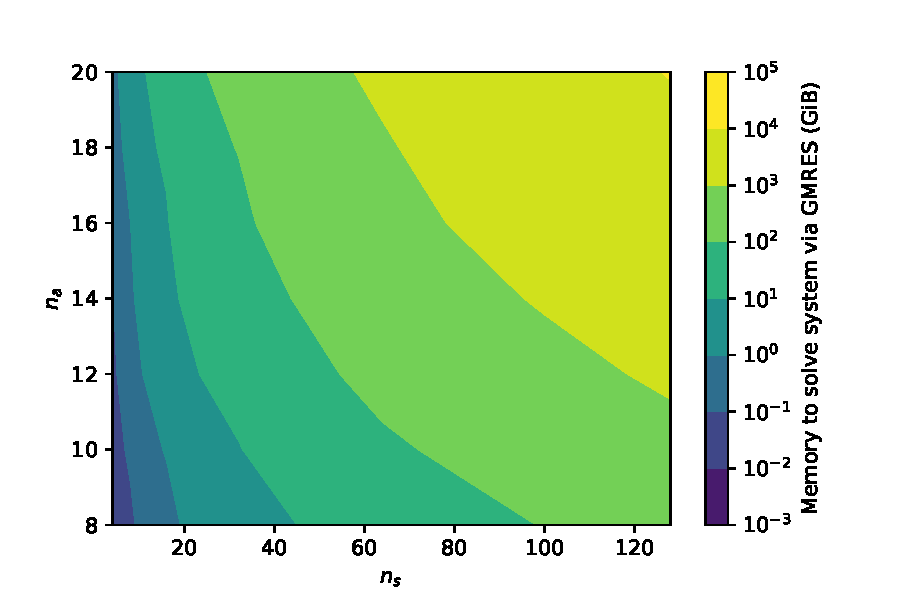
\includegraphics[width=5in]{memory_solve}
  \caption{Memory to solve the linear system of equations with GMRES restarted every 100 iterations. This seems to require roughly five times the memory required to store the matrix.}
  \label{fig:memory_solve}
\end{figure}


\section{Rules of Thumb}
\subsection{Grid Size and Discretization Error}
\subsection{Optical Conditions for Asymptotics}

\begin{figure}[H]
  \centering
  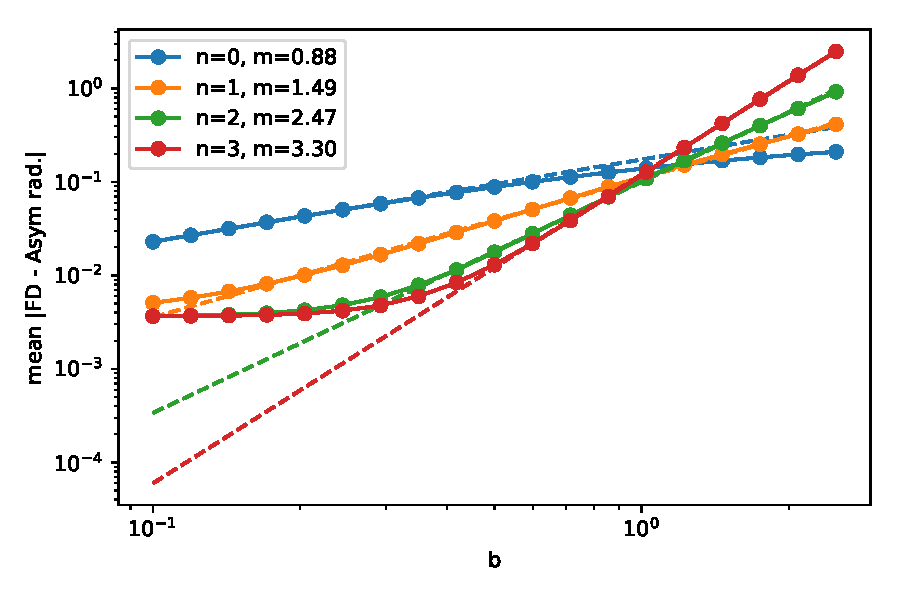
\includegraphics[width=5in]{verify_real_kelp_asym_b_scat_ss_sm_th_a05_br01_72x10_rad_err}
  \caption{Asym real kelp. Blur radius=0.1}
  \label{fig:asym_real_kelp_br01}
\end{figure}


\begin{figure}[H]
  \centering
  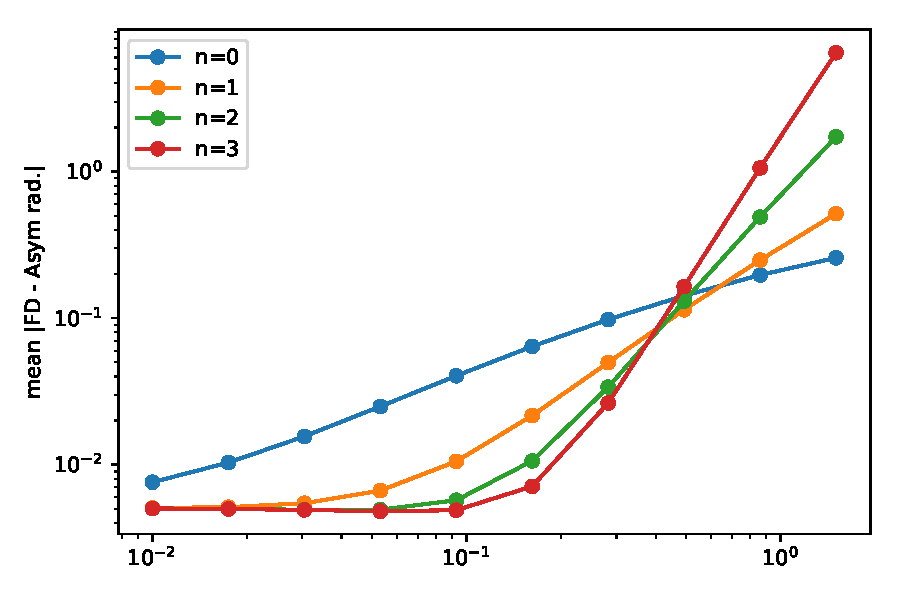
\includegraphics[width=5in]{asym_err_vs_b_a01}
  \caption{asym err vs b a01}
  \label{fig:asym_err_vs_b_a01}
\end{figure}

\begin{figure}[H]
  \centering
  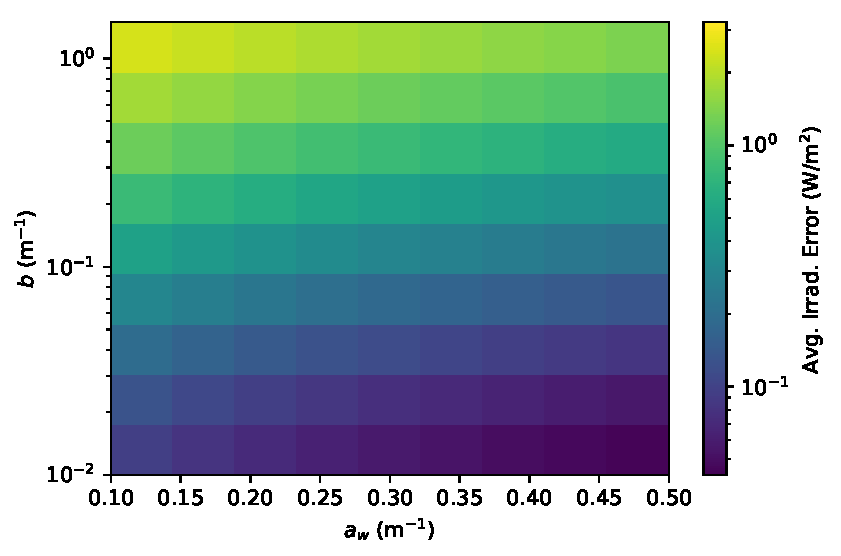
\includegraphics[width=5in]{asym_err_vs_ab}
  \caption{asym err vs ab}
  \label{fig:asym_err_vs_ab}
\end{figure}

\begin{figure}[H]
  \centering
  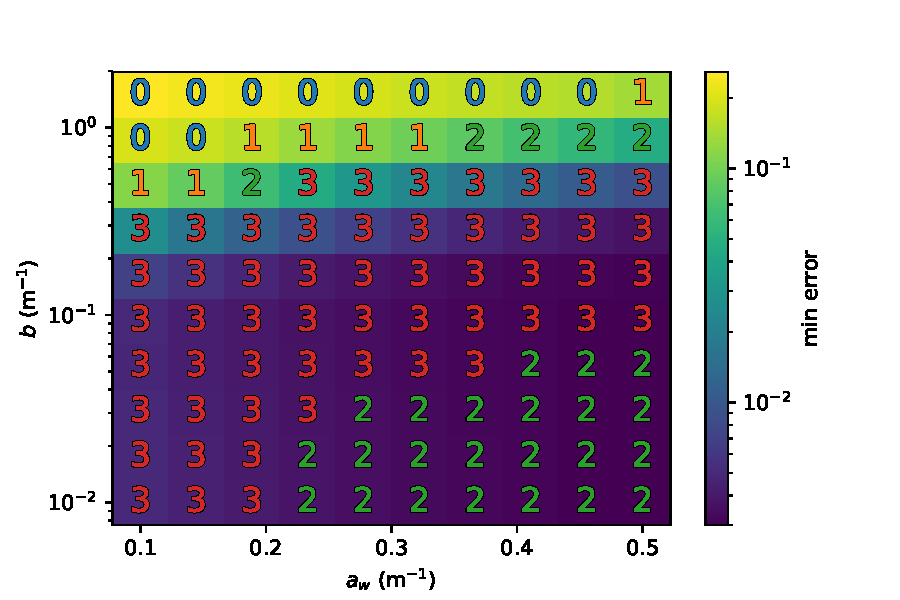
\includegraphics[width=5in]{best_n_data_vs_ab}
  \caption{best n data vs ab}
  \label{fig:best_n_data_vs_ab}
\end{figure}

\begin{figure}[H]
  \centering
  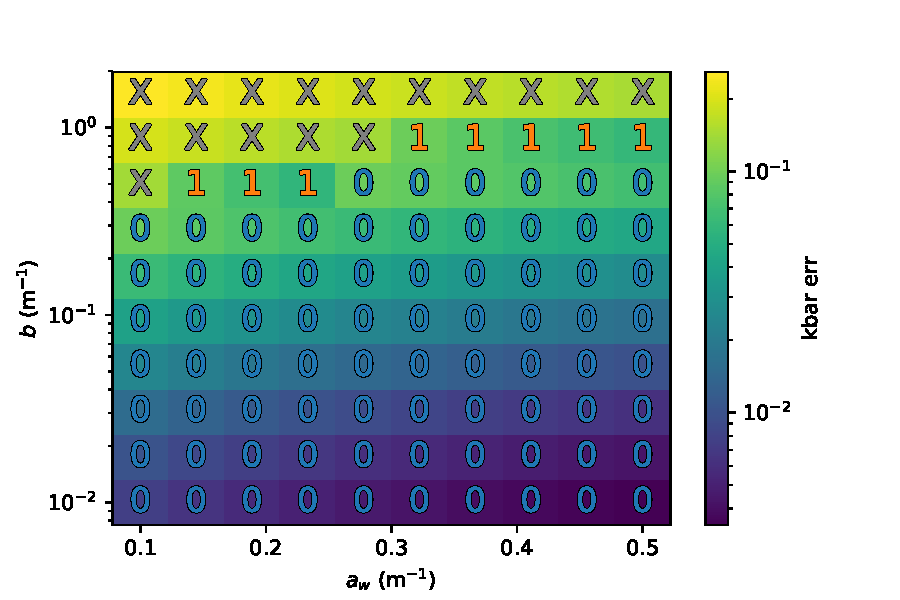
\includegraphics[width=5in]{min_n_data_vs_ab_eps01}
  \caption{min n data vs ab eps01}
  \label{fig:min_n_data_vs_ab_eps01}
\end{figure}

\begin{figure}[H]
  \centering
  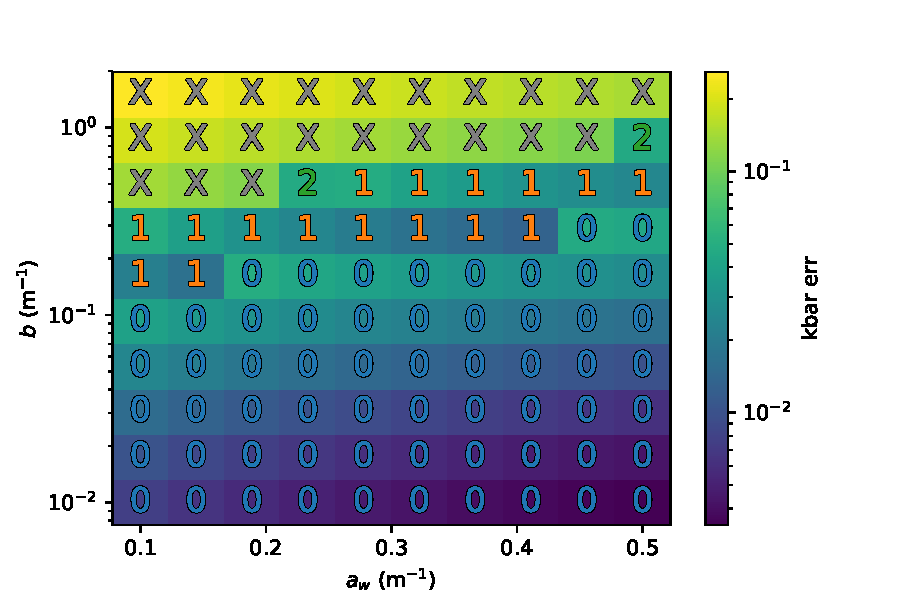
\includegraphics[width=5in]{min_n_data_vs_ab_eps005}
  \caption{min n data vs ab eps005}
  \label{fig:min_n_data_vs_ab_eps005}
\end{figure}

\begin{figure}[H]
  \centering
  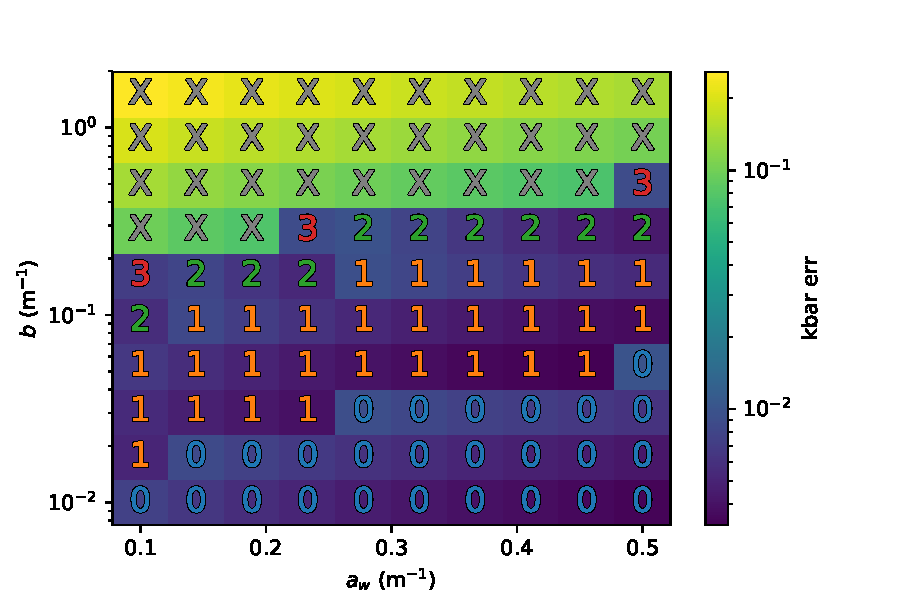
\includegraphics[width=5in]{min_n_data_vs_ab_eps001}
  \caption{min n data vs ab eps001}
  \label{fig:min_n_data_vs_ab_eps001}
\end{figure}

\begin{figure}[H]
  \centering
  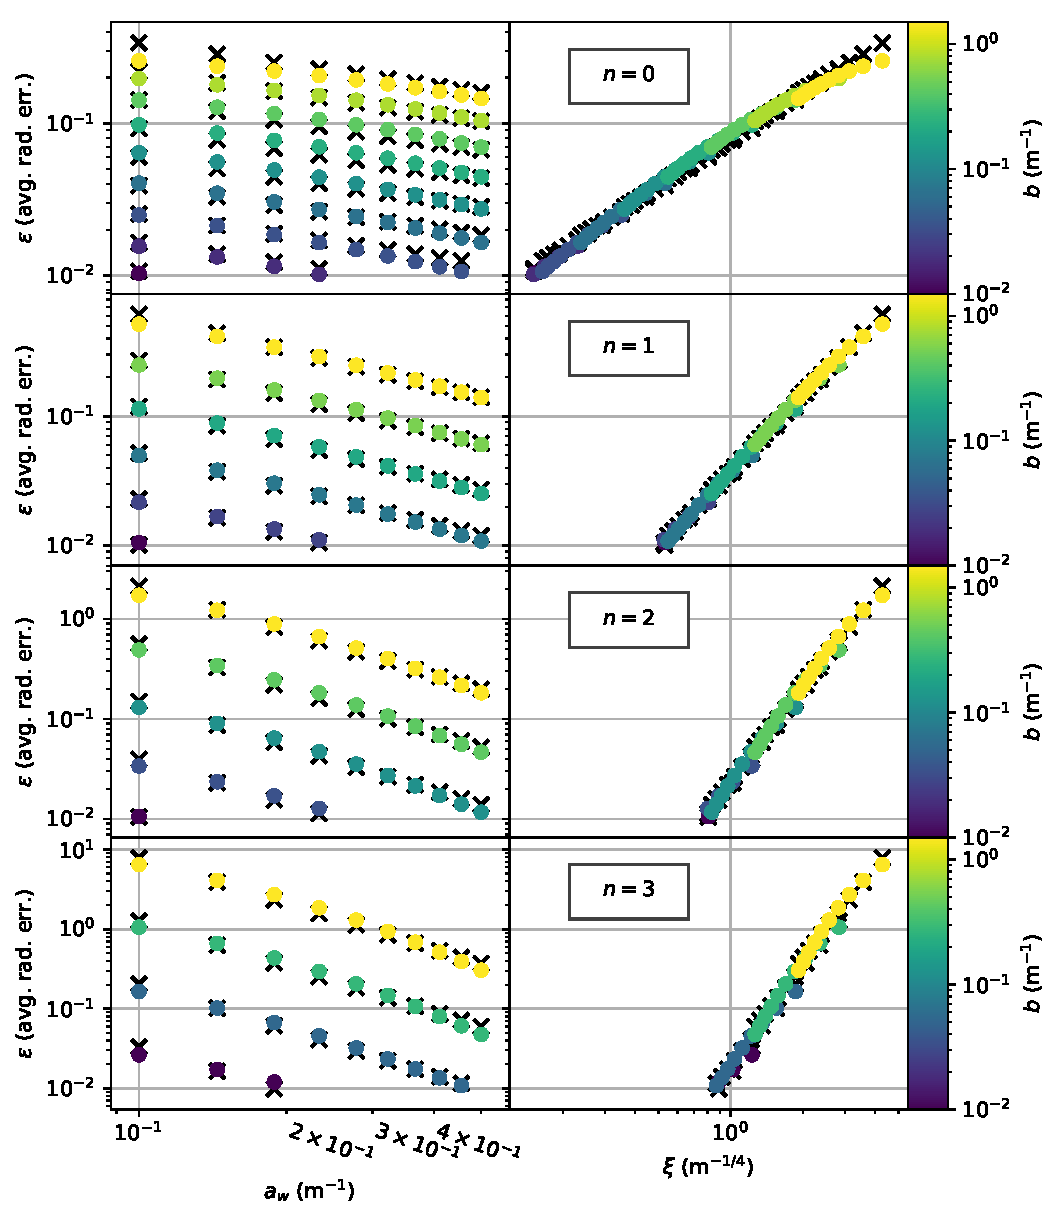
\includegraphics[width=6in]{asym_err_data_xi_model}
  \caption{asym err data xi model}
  \label{fig:asym_err_data_xi_model}
\end{figure}

\begin{figure}[H]
  \centering
  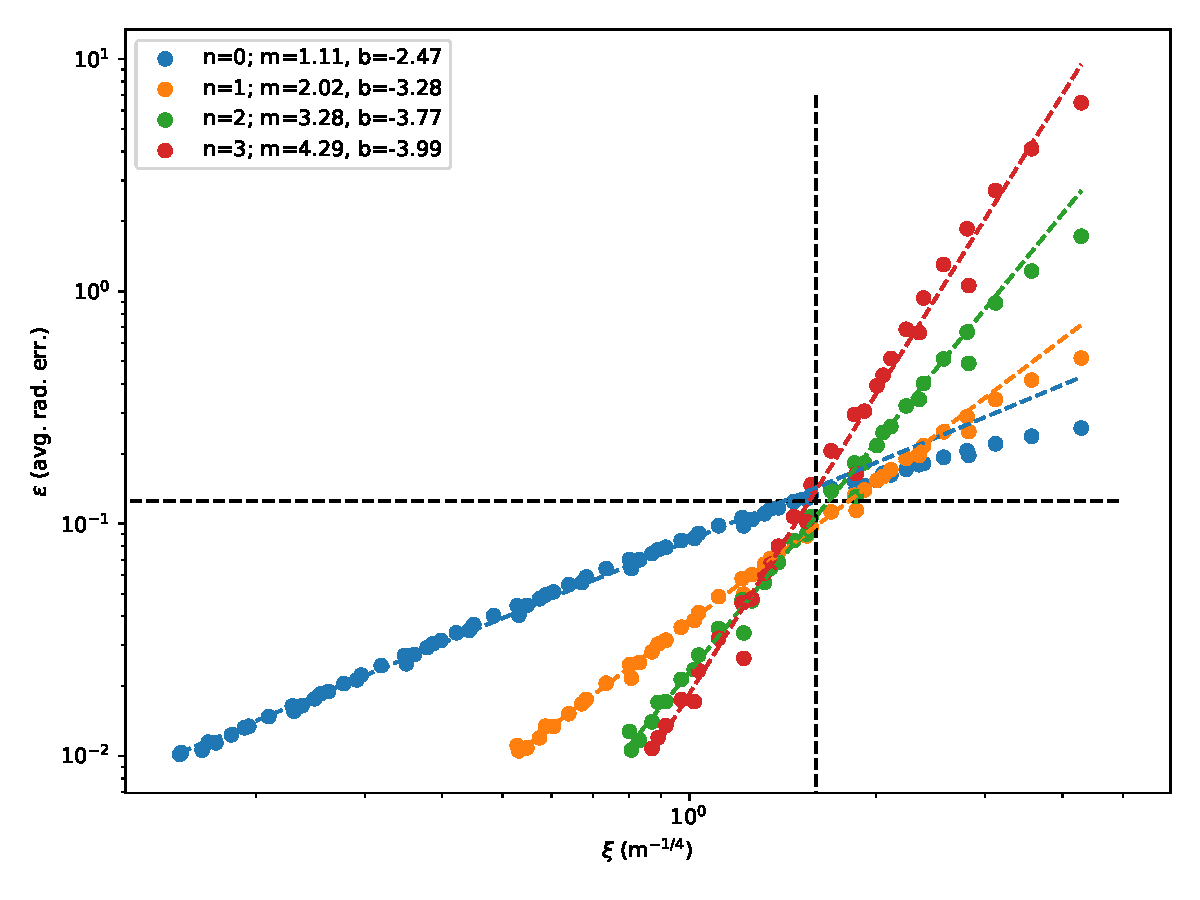
\includegraphics[width=5in]{asym_err_vs_x_all_n_fit_all}
  \caption{asym err vs x all n fit all}
  \label{fig:asym_err_vs_x_all_n_fit_all}
\end{figure}

\begin{figure}[H]
  \centering
  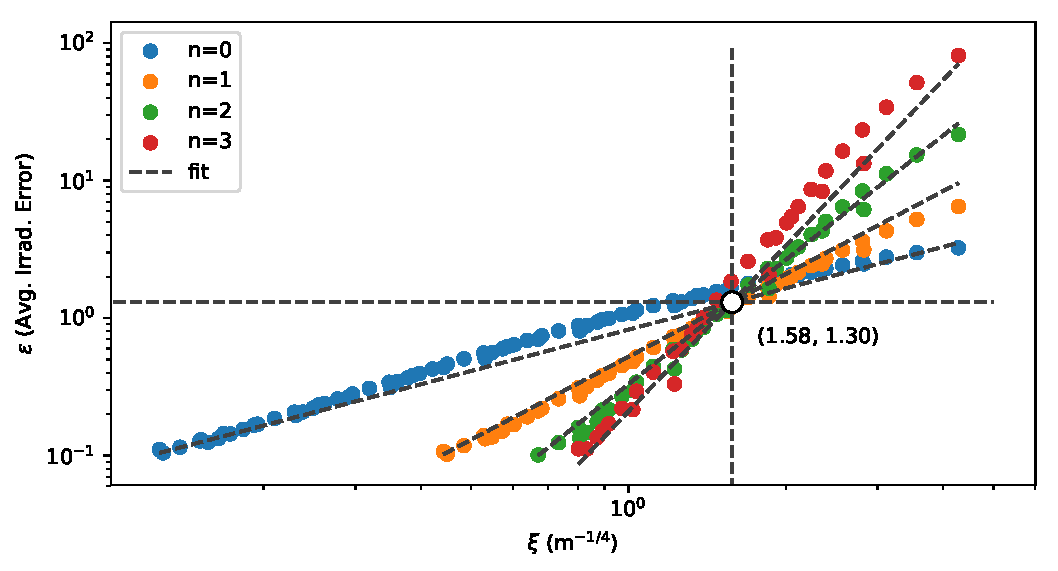
\includegraphics[width=5in]{asym_err_vs_xi_all_n_fit_all}
  \caption{asym err vs xi all n fit all}
  \label{fig:asym_err_vs_xi_all_n_fit_all}
\end{figure}

\begin{figure}[H]
  \centering
  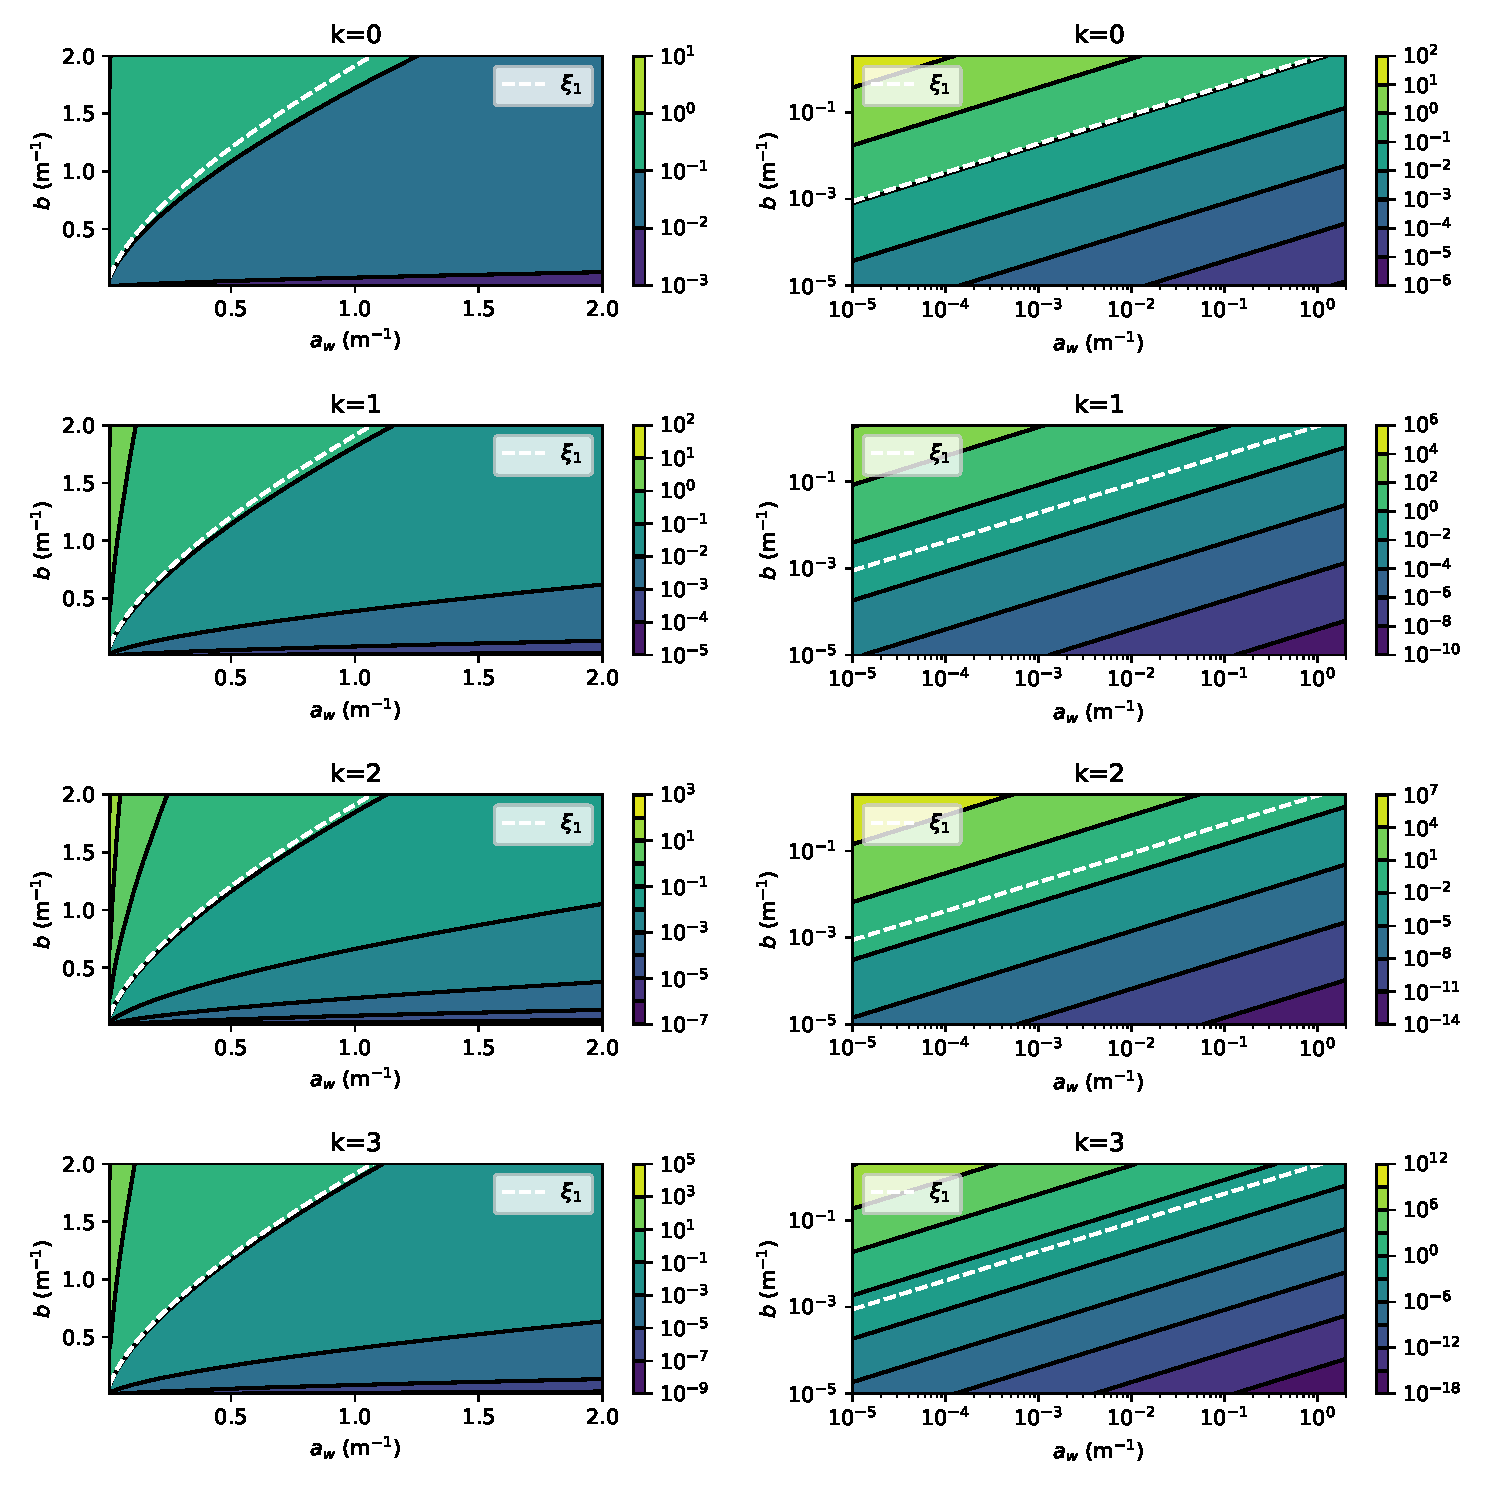
\includegraphics[width=5in]{asym_err_model_vs_ab_all_k}
  \caption{asym err model vs ab all k}
  \label{fig:asym_err_model_vs_ab_all_k}
\end{figure}

\begin{figure}[H]
  \centering
  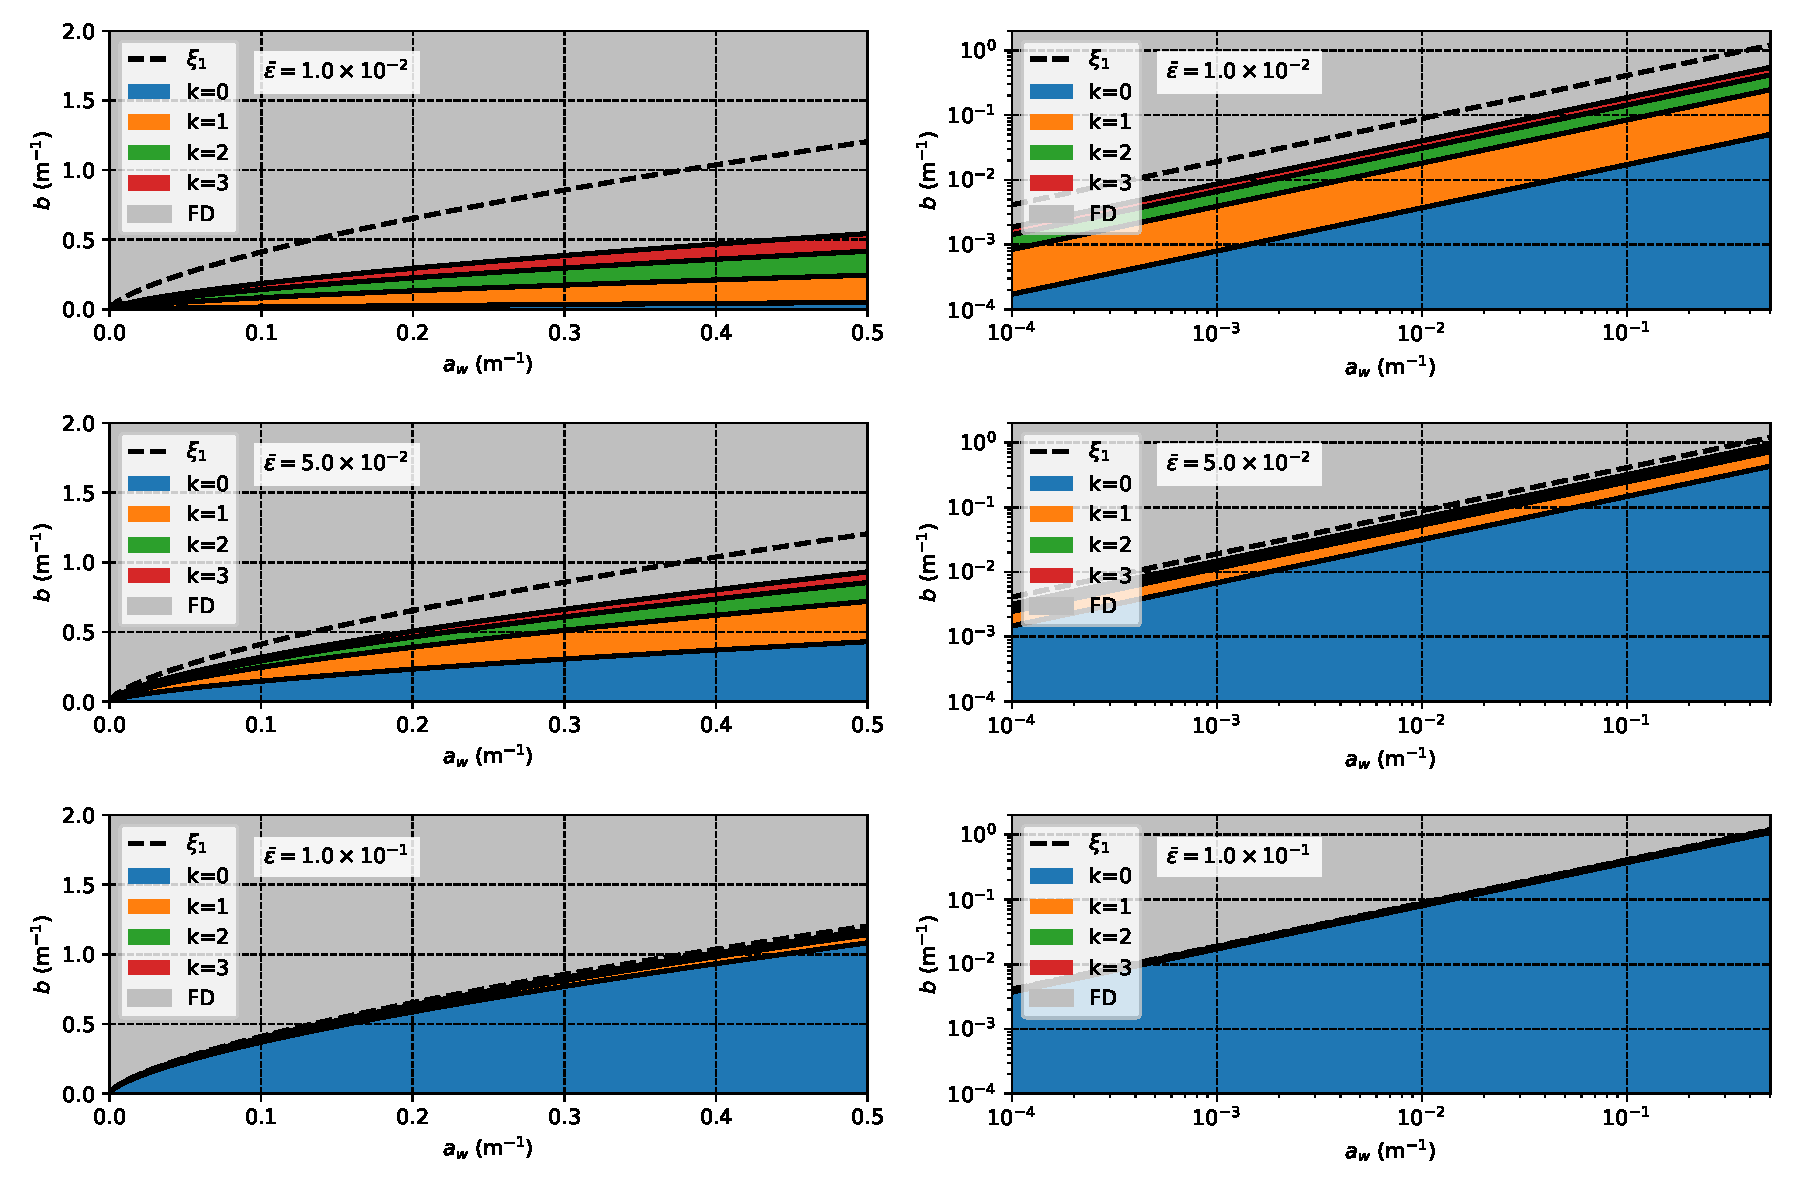
\includegraphics[width=5in]{nbar_model_vs_ab_3eps}
  \caption{nbar model vs ab 3eps}
  \label{fig:nbar_model_vs_ab_3eps}
\end{figure}

\begin{figure}[H]
  \centering
  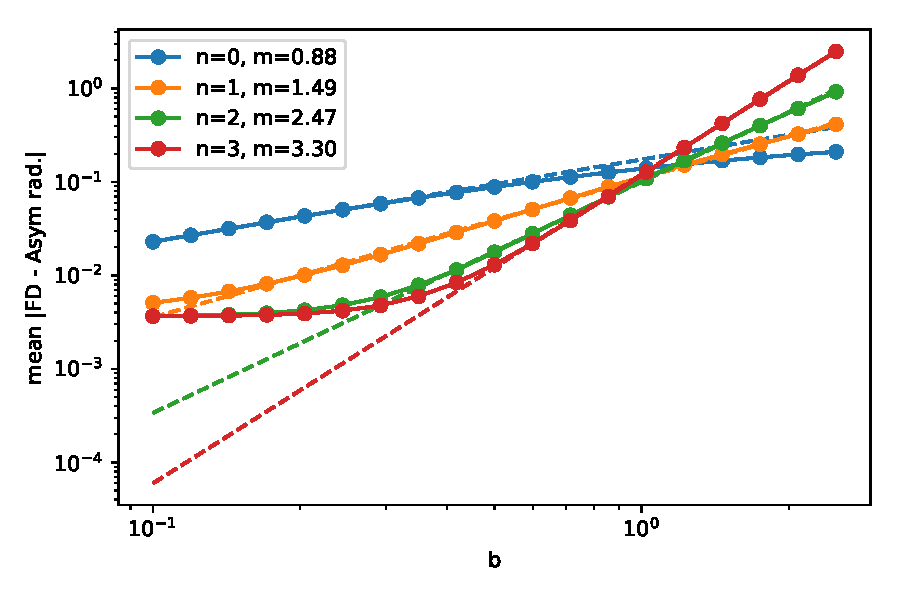
\includegraphics[width=5in]{verify_real_kelp_asym_b_scat_ss_sm_th_a05_br01_72x10_rad_err}
  \caption{Asym real kelp. Blur radius=0.1}
  \label{fig:asym_real_kelp_br01}
\end{figure}

\section{Comparison to Other Light Models}


\subsection{Full 10m}
\begin{figure}[H]
  \centering
  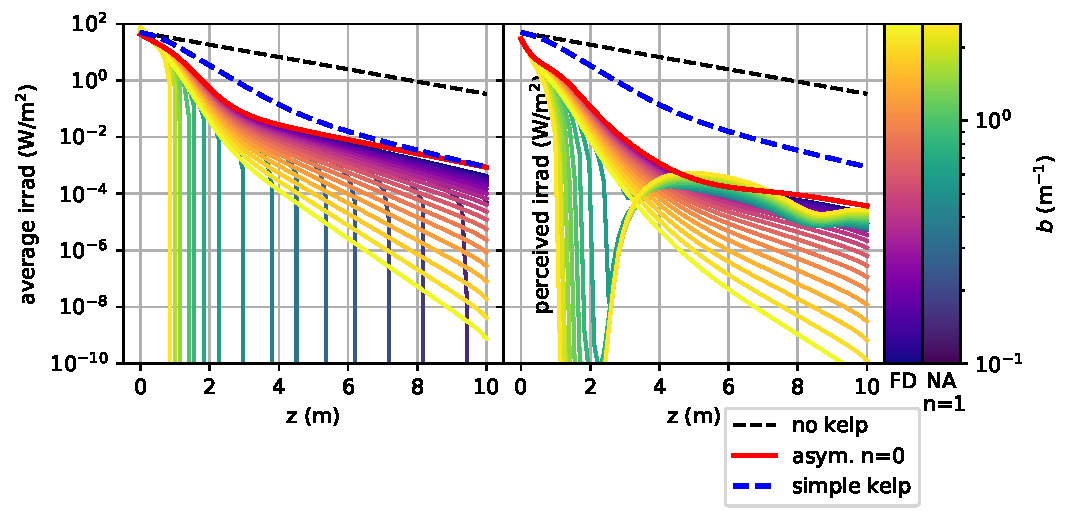
\includegraphics[width=6in]{compare_models_n1}
  \caption{Compare models n=1}
  \label{fig:compare_models_n1}
\end{figure}
\begin{figure}[H]
  \centering
  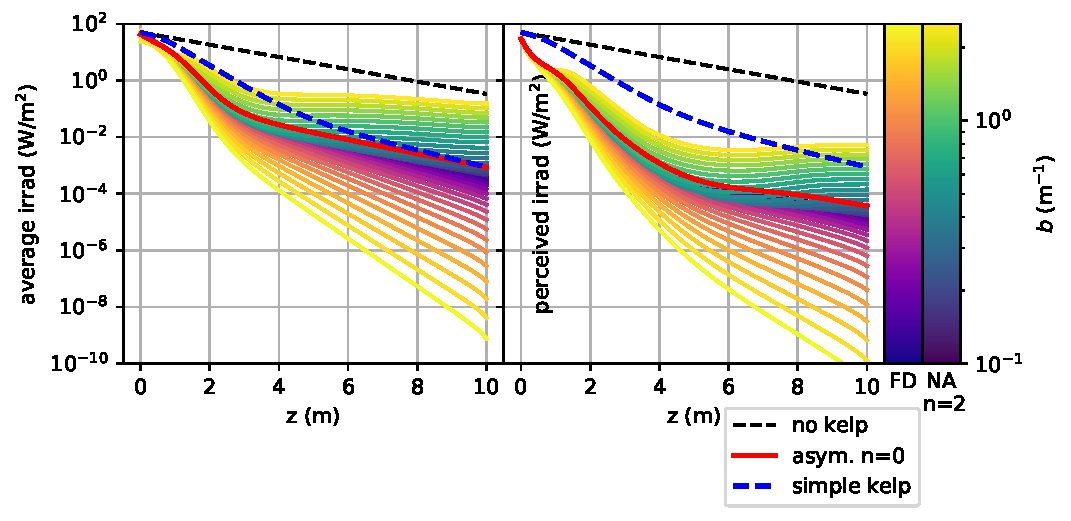
\includegraphics[width=6in]{compare_models_n2}
  \caption{Compare models n=2}
  \label{fig:compare_models_n2}
\end{figure}
\begin{figure}[H]
  \centering
  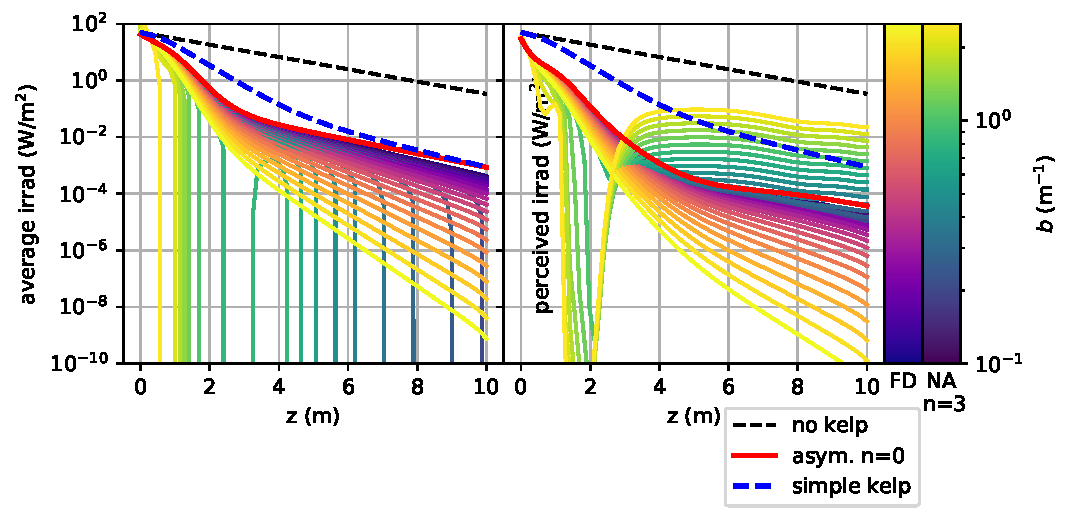
\includegraphics[width=6in]{compare_models_n3}
  \caption{Compare models n=3}
  \label{fig:compare_models_n3}
\end{figure}

\subsection{First 4m}
\begin{figure}[H]
  \centering
  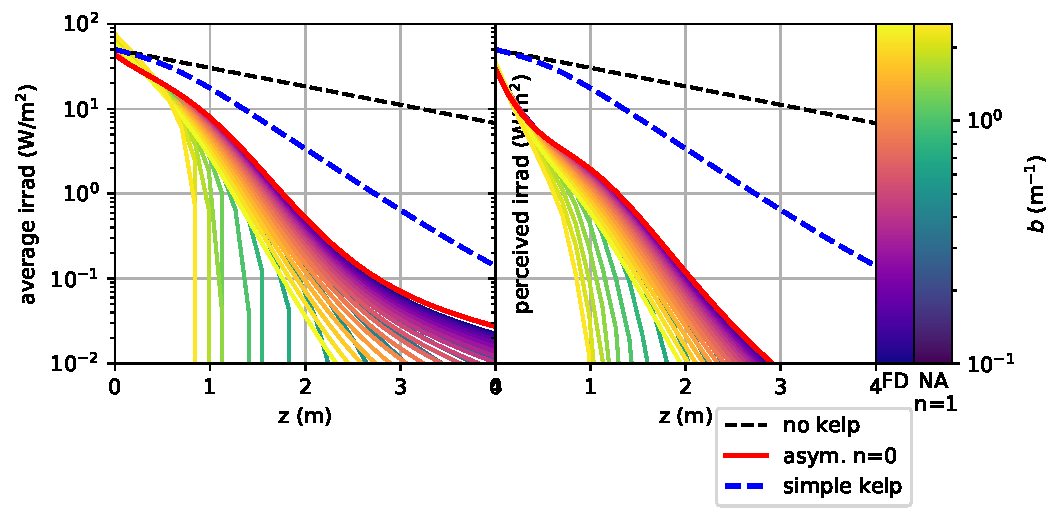
\includegraphics[width=6in]{compare_models_n1_zoom}
  \caption{Compare models n=1}
  \label{fig:compare_models_n1}
\end{figure}
\begin{figure}[H]
  \centering
  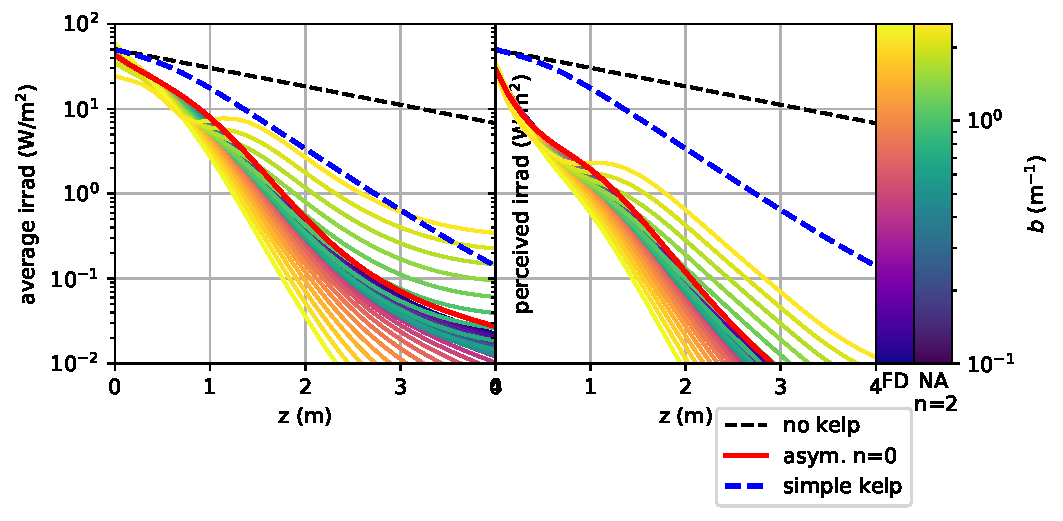
\includegraphics[width=6in]{compare_models_n2_zoom}
  \caption{Compare models n=2}
  \label{fig:compare_models_n2}
\end{figure}
\begin{figure}[H]
  \centering
  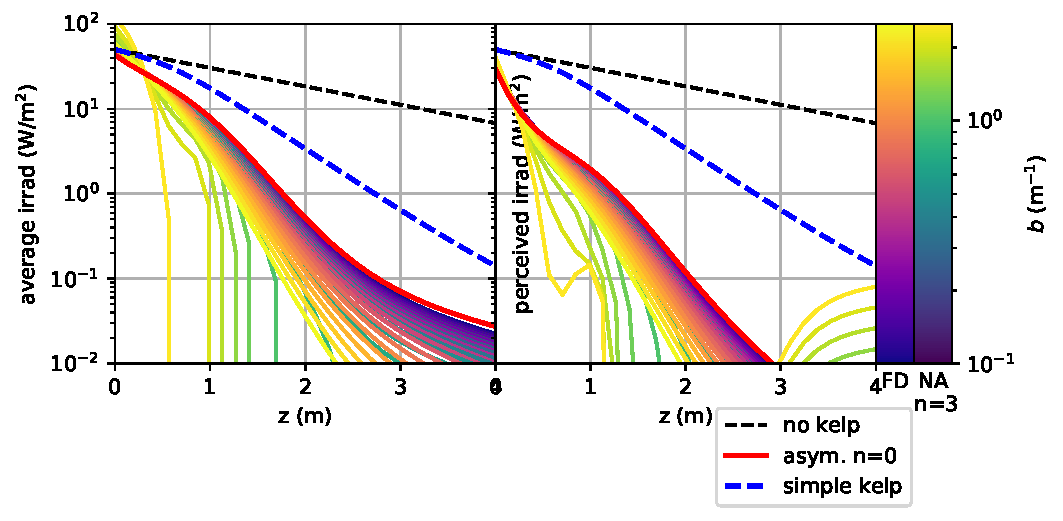
\includegraphics[width=6in]{compare_models_n3_zoom}
  \caption{Compare models n=3}
  \label{fig:compare_models_n3}
\end{figure}

\subsection{First 2m}
\begin{figure}[H]
  \centering
  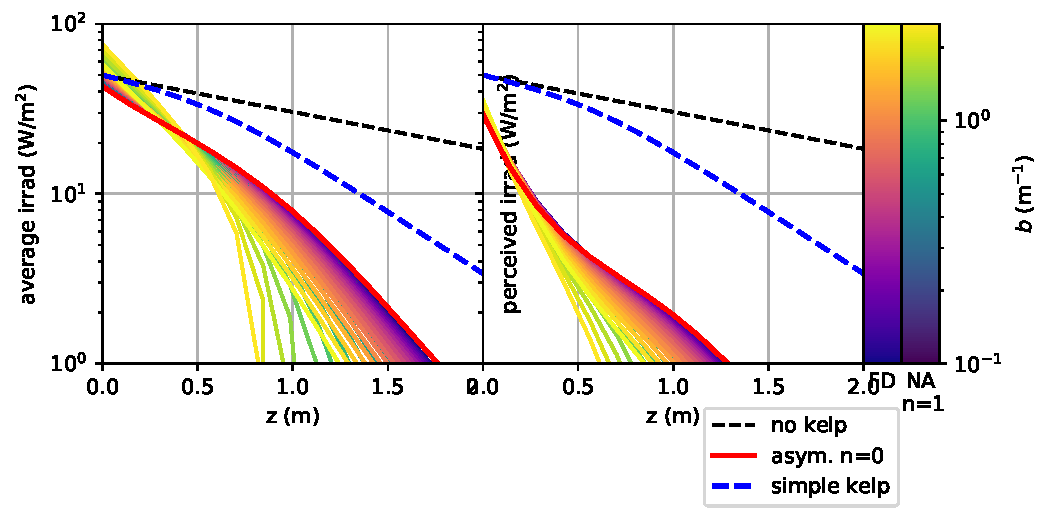
\includegraphics[width=6in]{compare_models_n1_zoom2}
  \caption{Compare models n=1}
  \label{fig:compare_models_n1}
\end{figure}
\begin{figure}[H]
  \centering
  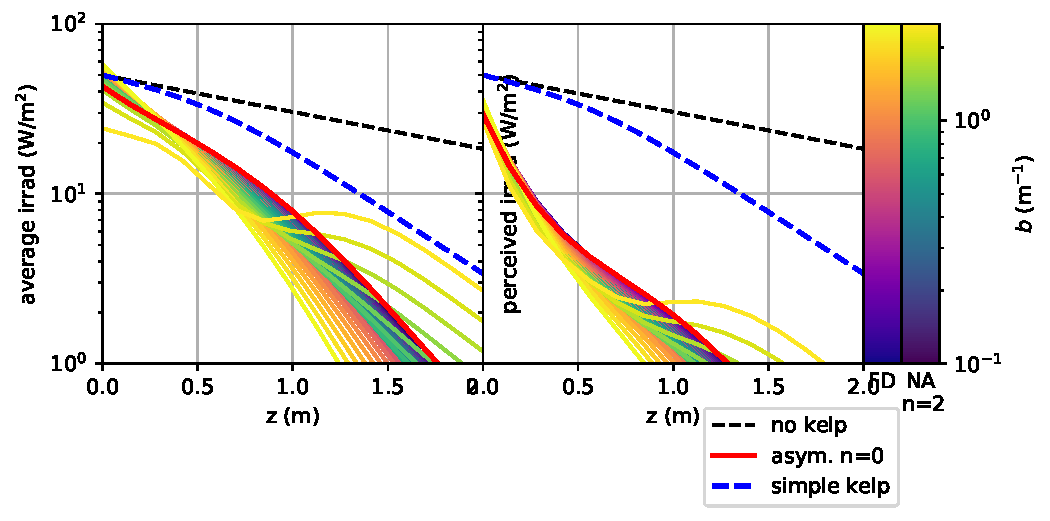
\includegraphics[width=6in]{compare_models_n2_zoom2}
  \caption{Compare models n=2}
  \label{fig:compare_models_n2}
\end{figure}
\begin{figure}[H]
  \centering
  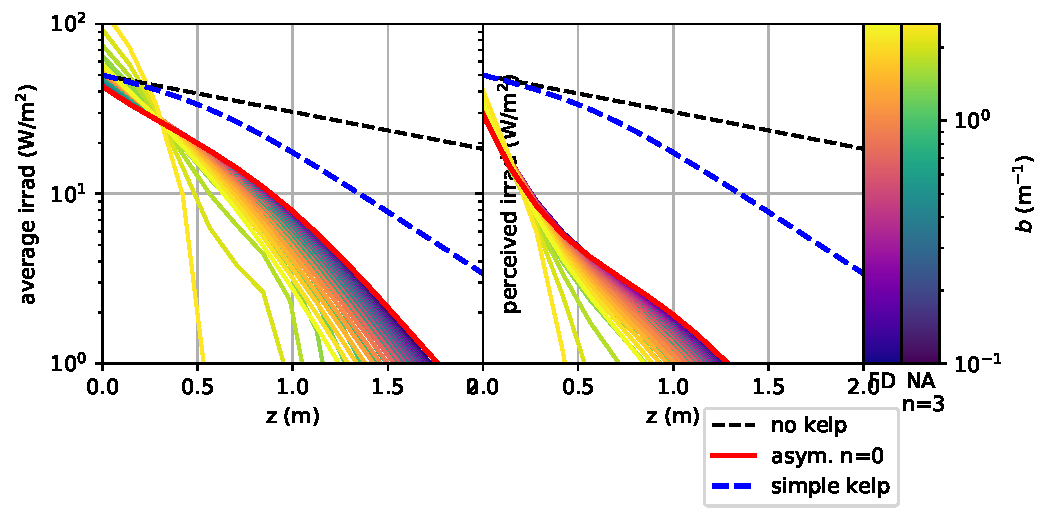
\includegraphics[width=6in]{compare_models_n3_zoom2}
  \caption{Compare models n=3}
  \label{fig:compare_models_n3}
\end{figure}
